\documentclass[tikz,border=6pt]{standalone}
% Shared preamble of the standalone figures: fonts as in the decks, the TikZ
% libraries, the notation, and the styles.
\usepackage[T1]{fontenc}
\usepackage[utf8]{inputenc}
\usepackage[sfdefault,lining]{FiraSans}
\usepackage{FiraMono}
\usepackage{amsmath}
\usetikzlibrary{positioning,arrows.meta,calc,shapes.misc,fit,backgrounds,
                decorations.pathreplacing,patterns,matrix}
% Notation for the MACE4D figures.
%
% Every parameter, symbol, default value, and constant that a figure shows is
% a macro here, so that the figures change from code names to symbols, or
% follow a change of a default, by editing this file alone.
%
%   \codenamestrue   renders each parameter as its code name (current setting)
%   \codenamesfalse  renders the symbolic form
%
% \sym{code name}{symbol} is the switch every parameter macro uses.  A
% parameter that exists on both models carries its owner in code mode.

\newif\ifcodenames
\codenamestrue

\providecommand{\code}[1]{\texttt{#1}}
\newcommand{\sym}[2]{\ifcodenames\code{#1}\else\ensuremath{#2}\fi}
\newcommand{\ctmodel}{\code{ct\_model}}
\newcommand{\macemodel}{\code{MACE4DModel}}
% A key line "code name <-> symbol", shown in code mode only.
\newcommand{\keyline}[2]{\ifcodenames#1~\ensuremath{\leftrightarrow}~\ensuremath{#2}\fi}

% ------------------------------------------------------------ math symbols
% These are always symbolic; the formulas use them, and the key lines tie
% them to the code names.
\newcommand{\symSigY}{\sigma_y}
\newcommand{\symSigProx}{\sigma_p}
\newcommand{\symSigNoise}{\sigma_n}
\newcommand{\symSigX}{\sigma_x}
\newcommand{\symSharpness}{s}
\newcommand{\symBeta}[1]{\beta_{#1}}
\newcommand{\symRho}{\rho}
\newcommand{\symNbrWeightTime}{b_t}
\newcommand{\symNumFrames}{T}
\newcommand{\symFramesPerRotation}{P}
\newcommand{\symOverlap}{f}

% ------------------------------------------------------------------ objects
\newcommand{\frameCube}[1]{\ensuremath{C_{#1}}}          % frame t of the 4D image
\newcommand{\fourD}{\ensuremath{x}}                      % the 4D image
\newcommand{\initImage}{\ensuremath{x^{0}}}              % the initial 4D image
\newcommand{\sinoFrame}[1]{\ensuremath{y_{#1}}}          % the views of frame t
\newcommand{\weightsFrame}[1]{\ensuremath{\Lambda_{#1}}} % the weights of frame t
\newcommand{\projFrame}[1]{\ensuremath{A_{#1}}}          % the frame model
\newcommand{\proxAgent}[1]{\ensuremath{F_{#1}}}          % the prox map of frame t
\newcommand{\dataFitAgent}{\ensuremath{F}}               % all frames' prox maps as one agent
\newcommand{\orientXY}{\sym{XY-t}{\mathrm{XY}t}}
\newcommand{\orientYZ}{\sym{YZ-t}{\mathrm{YZ}t}}
\newcommand{\orientXZ}{\sym{XZ-t}{\mathrm{XZ}t}}
\newcommand{\denoiser}[1]{\ensuremath{G_{#1}}}           % \denoiser{\orientXY}
\newcommand{\stateW}[1]{\ensuremath{W_{#1}}}             % the loop's input to agent k
\newcommand{\outX}[1]{\ensuremath{X_{#1}}}               % the output of agent k
\newcommand{\avgZ}{\ensuremath{z}}
\newcommand{\xbar}{\ensuremath{\bar{x}}}
\newcommand{\filterMatrix}{\sym{filter\_matrix}{H}}
\newcommand{\genInit}{\code{'init'}}                     % the generator of the partitions
\newcommand{\genIteration}{the iteration number}          % the generator of the subset order

% --------------------------------------------- parameters and their defaults
% Scan and frames (constructor arguments of MACE4DModel)
\newcommand{\pFramesPerRotation}{\sym{frames\_per\_rotation}{\symFramesPerRotation}}
\newcommand{\defFramesPerRotation}{6}
\newcommand{\pFrameOverlapFactor}{\sym{frame\_overlap\_factor}{\symOverlap}}
\newcommand{\defFrameOverlapFactor}{2.0}
\newcommand{\pNumFrames}{\sym{num\_frames}{\symNumFrames}}
\newcommand{\defNumFrames}{all}

% Set on ct_model; reach the frame models
\newcommand{\pSnrDb}{\sym{snr\_db}{\mathrm{SNR}_{\mathrm{dB}}}}
\newcommand{\defSnrDb}{30}
\newcommand{\pSharpnessCt}{\sym{ct\_model.sharpness}{\symSharpness_{\mathrm{ct}}}}
\newcommand{\defSharpnessCt}{1.0}
\newcommand{\pSigmaProxCt}{\sym{ct\_model.sigma\_prox}{\symSigProx^{\mathrm{ct}}}}
\newcommand{\pSigmaXCt}{\sym{ct\_model.sigma\_x}{\symSigX^{\mathrm{ct}}}}
\newcommand{\pPQTCt}{\sym{ct\_model.p, q, T}{(p, q, T)_{\mathrm{ct}}}}
\newcommand{\pSigmaY}{\sym{sigma\_y}{\symSigY}}

% Set on MACE4DModel
\newcommand{\pSigmaProxMace}{\sym{MACE4DModel.sigma\_prox}{\symSigProx}}
\newcommand{\defSigmaProxMace}{None (estimated per frame)}
\newcommand{\pSigmaNoise}{\sym{sigma\_noise}{\symSigNoise}}
\newcommand{\defSigmaNoise}{None (estimated)}
\newcommand{\pSigmaXMace}{\sym{MACE4DModel.sigma\_x}{\symSigX}}
\newcommand{\defSigmaXMace}{estimated}
\newcommand{\pSharpnessMace}{\sym{MACE4DModel.sharpness}{\symSharpness}}
\newcommand{\defSharpnessMace}{0.0}
\newcommand{\pPQTMace}{\sym{MACE4DModel.p, q, T}{(p, q, T)}}
\newcommand{\defPQT}{2.0, 1.2, 1.0}
\newcommand{\pNbrWeightTime}{\sym{nbr\_weight\_time}{\symNbrWeightTime}}
\newcommand{\defNbrWeightTime}{1.0}
\newcommand{\pMacePriorWeight}{\sym{mace\_prior\_weight}{\beta}}
\newcommand{\defMacePriorWeight}{0.5}
\newcommand{\pRhoMann}{\sym{rho\_mann}{\symRho}}
\newcommand{\defRhoMann}{0.5}
\newcommand{\pProxNumIterations}{\sym{prox\_num\_iterations}{N_p}}
\newcommand{\defProxNumIterations}{3}
\newcommand{\pProxPartitionAdvance}{\sym{prox\_partition\_advance}{a}}
\newcommand{\defProxPartitionAdvance}{1.0}
\newcommand{\pProxWarmStart}{\code{prox\_warm\_start}}
\newcommand{\defProxWarmStart}{True}
\newcommand{\pProxStopThreshold}{\code{prox\_stop\_threshold}}
\newcommand{\defProxStopThreshold}{0.02}
\newcommand{\pDenoiserWarmStart}{\code{denoiser\_warm\_start}}
\newcommand{\defDenoiserWarmStart}{False}
\newcommand{\pDenoiseSlabGb}{\code{denoise\_slab\_gb}}
\newcommand{\defDenoiseSlabGb}{2.0}
\newcommand{\pDejitter}{\code{dejitter}}
\newcommand{\defDejitter}{True}
\newcommand{\pDevicePool}{\code{set\_device\_pool}}
\newcommand{\pNumDevicesEnv}{\code{MBIRTORCH\_NUM\_DEVICES}}

% Arguments of MACE4DModel.recon
\newcommand{\pMaxIterations}{\sym{max\_iterations}{N}}
\newcommand{\defMaxIterations}{10}
\newcommand{\pStopThreshold}{\code{stop\_threshold\_change\_pct}}
\newcommand{\defStopThreshold}{0.2}
\newcommand{\pSeed}{\code{seed}}
\newcommand{\defSeed}{None}
\newcommand{\pInitRecon}{\code{init\_recon}}
\newcommand{\pInitDir}{\code{init\_dir}}

% ---------------------------------------------------------------- constants
\newcommand{\cInitIterations}{15}        % iterations of the per-frame initial image
\newcommand{\cDenoiseMaxIterations}{15}  % iterations per denoised volume, at most
\newcommand{\cDenoiseStopPct}{0.05}      % percent change that stops a denoised volume
\newcommand{\cSigmaXFactor}{0.2}         % sigma_x and sigma_prox estimates: factor * 2^sharpness * std
\newcommand{\cSigmaXFloor}{10^{-6}}      % floor of the denoiser sigma_x estimate
\newcommand{\cSigmaXBase}{1.0}           % base default of sigma_x when no estimate runs
\newcommand{\cDenoiseSubsets}{16}        % pixel subsets of a denoiser partition, at most
\newcommand{\cPixelsPerSubset}{64}       % fewer pixels per subset than this and the count drops

% ------------------------------------------- symbols the figures use inline
\newcommand{\symPriorWeight}{\ensuremath{w}}    % the value of the prior weight
\newcommand{\symFilterMatrix}{\ensuremath{H}}   % the temporal filter
\newcommand{\symFrameIndex}{\ensuremath{t}}
\newcommand{\symNumDevices}{\ensuremath{n}}     % the size of the device pool
\newcommand{\degsym}{\ensuremath{^{\circ}}}
% Argument values of the device pool selector
\newcommand{\valNone}{\code{None}}
\newcommand{\valCpu}{\code{'cpu'}}
\newcommand{\valGpu}{\code{'gpu'}}
% Derived defaults, in degrees (integers; add rounding if a default ever gives a fraction)
\newcommand{\defFrameStepDeg}{\pgfmathparse{int(360/\defFramesPerRotation)}\pgfmathresult}
\newcommand{\defFrameSpanDeg}{\pgfmathparse{int(\defFrameOverlapFactor*360/\defFramesPerRotation)}\pgfmathresult}
% Axis labels of the 4D image
\newcommand{\axisT}{\ensuremath{t}}
\newcommand{\axisX}{\ensuremath{x}}
\newcommand{\axisY}{\ensuremath{y}}
\newcommand{\axisZ}{\ensuremath{z}}

% Colors and TikZ styles shared by the MACE4D figures.
%
% Blue is the data-fit side, green the priors, amber the consensus state.
% A solid arrow carries a value the user set; a dashed arrow carries an
% estimate.  \cube draws one frame of the 4D image.

\definecolor{datafitBlue}{HTML}{3D6B99}
\definecolor{priorGreen}{HTML}{2E7D32}
\definecolor{stateAmber}{HTML}{B26B1F}
\definecolor{warnRed}{HTML}{A23B3B}
\definecolor{inkGray}{HTML}{5A5A5A}
\definecolor{lineGray}{HTML}{9A9A9A}
\definecolor{paleBlue}{HTML}{E3ECF5}
\definecolor{paleGreen}{HTML}{E4F0E4}
\definecolor{paleAmber}{HTML}{F5EBDD}
\definecolor{paleGray}{HTML}{F0F0F0}

\tikzset{
  every node/.style={font=\small},
  box/.style={draw, rounded corners=3pt, thick, align=center, inner sep=5pt,
              minimum height=8mm},
  datafit/.style={box, draw=datafitBlue, fill=paleBlue},
  prior/.style={box, draw=priorGreen, fill=paleGreen},
  state/.style={box, draw=stateAmber, fill=paleAmber},
  plain/.style={box, draw=lineGray, fill=paleGray},
  note/.style={font=\footnotesize, text=inkGray, align=left},
  notebox/.style={note, draw=lineGray, rounded corners=2pt, inner sep=4pt,
                  fill=white},
  param/.style={font=\footnotesize, align=left},
  title/.style={font=\bfseries, align=left},
  setarrow/.style={-{Stealth[length=2mm]}, thick},
  estarrow/.style={-{Stealth[length=2mm]}, thick, dashed, inkGray},
  flow/.style={-{Stealth[length=2mm]}, semithick},
  flowblue/.style={flow, datafitBlue},
  flowgreen/.style={flow, priorGreen},
  flowamber/.style={flow, stateAmber},
  cut/.style={-{Stealth[length=1.5mm]}, thin, inkGray},
  cubeFront/.style={fill=white, draw=black!70, thin},
  cubeTop/.style={fill=black!8, draw=black!70, thin},
  cubeSide/.style={fill=black!20, draw=black!70, thin},
}

% \cube{x}{y}{size}{label}: a cube whose front face has its lower left
% corner at (x, y) and side length size, with a label on the front face.
\newcommand{\cube}[4]{%
  \begin{scope}[shift={(#1,#2)}]
    \pgfmathsetmacro{\cubeDepth}{0.35*#3}
    \draw[cubeTop] (0,#3) -- (\cubeDepth,#3+\cubeDepth) -- (#3+\cubeDepth,#3+\cubeDepth) -- (#3,#3) -- cycle;
    \draw[cubeSide] (#3,0) -- (#3+\cubeDepth,\cubeDepth) -- (#3+\cubeDepth,#3+\cubeDepth) -- (#3,#3) -- cycle;
    \draw[cubeFront] (0,0) rectangle (#3,#3);
    \node at (0.5*#3,0.5*#3) {#4};
  \end{scope}}

% \arrowkey{x}{y}: the legend of the two arrow kinds, anchored at (x, y).
\newcommand{\arrowkey}[2]{%
  \draw[setarrow] (#1,#2) -- ++(1,0) node[note, right] {set by the user};
  \draw[estarrow] (#1,#2-0.45) -- ++(1,0) node[note, right] {estimated from the data};}



\begin{document}
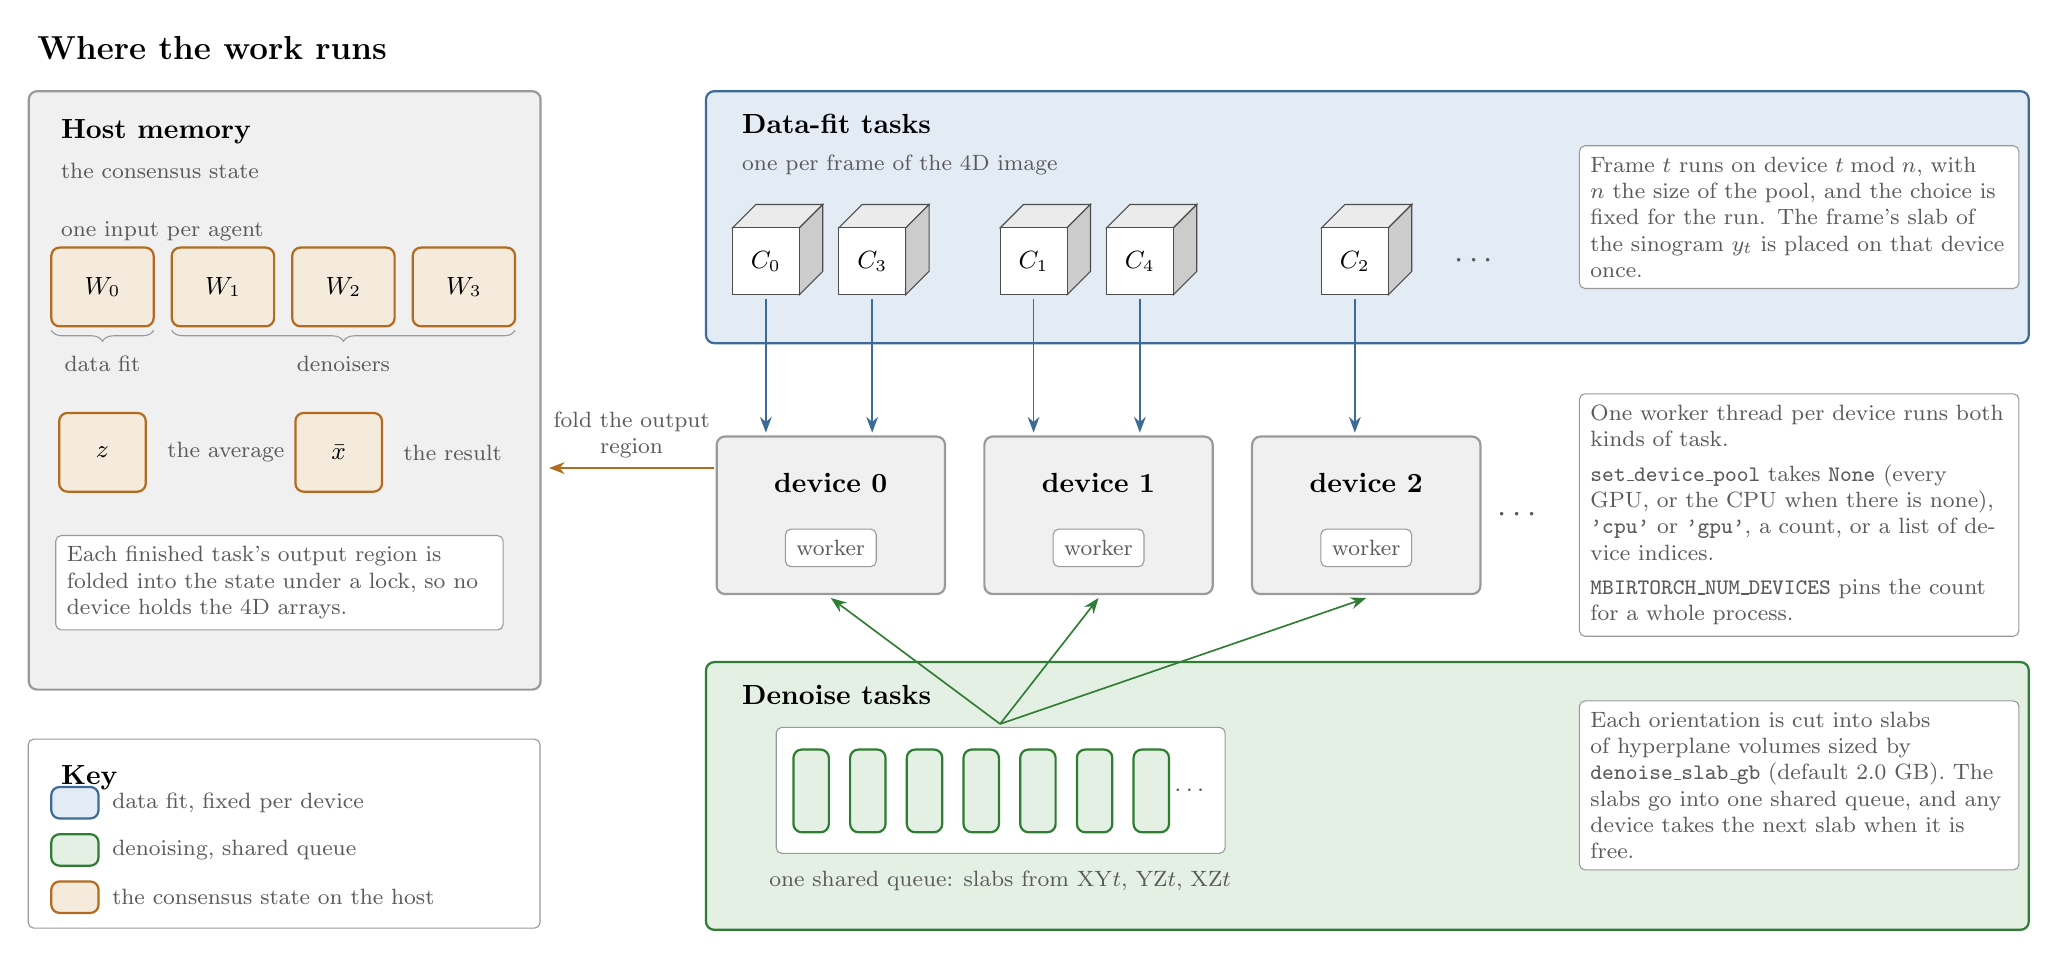
\begin{tikzpicture}

% ---------------------------------------------------------------- the title
\node[title, font=\large\bfseries, anchor=north west] at (0,13.0)
  {Where the work runs};

% ------------------------------------------------- the host and its state
\node[plain, anchor=north west, minimum width=65mm, minimum height=76mm]
  at (0,12.2) {};
\node[title, anchor=north west] at (0.3,11.95) {Host memory};
\node[note, anchor=north west] at (0.3,11.4) {the consensus state};

\node[note, anchor=north west] at (0.3,10.65) {one input per agent};
\foreach \k/\x in {0/0.95, 1/2.48, 2/4.01, 3/5.54}
  \node[state, minimum width=13mm, minimum height=10mm] at (\x,9.7) {\stateW{\k}};
\draw[lineGray, decorate, decoration={brace, mirror, amplitude=4pt}]
  (0.30,9.15) -- (1.60,9.15);
\draw[lineGray, decorate, decoration={brace, mirror, amplitude=4pt}]
  (1.83,9.15) -- (6.19,9.15);
\node[note, anchor=north] at (0.95,8.95) {data fit};
\node[note, anchor=north] at (4.01,8.95) {denoisers};

\node[state, minimum width=11mm, minimum height=10mm] at (0.95,7.6) {\avgZ};
\node[note, anchor=west] at (1.65,7.6) {the average};
\node[state, minimum width=11mm, minimum height=10mm] at (3.95,7.6) {\xbar};
\node[note, anchor=west] at (4.65,7.6) {the result};

\node[notebox, text width=5.4cm, anchor=north west] at (0.35,6.55)
  {Each finished task's output region is folded into the state under a lock,
   so no device holds the 4D arrays.};

% ------------------------------------------------------- the data-fit tasks
\node[datafit, anchor=north west, minimum width=168mm, minimum height=32mm]
  at (8.6,12.2) {};
\node[title, anchor=north west] at (8.95,12.02) {Data-fit tasks};
\node[note, anchor=north west] at (8.95,11.5) {one per frame of the 4D image};

% the frames, grouped over the device that runs them
\cube{8.95}{9.6}{0.85}{\frameCube{0}}
\cube{10.30}{9.6}{0.85}{\frameCube{3}}
\cube{12.35}{9.6}{0.85}{\frameCube{1}}
\cube{13.70}{9.6}{0.85}{\frameCube{4}}
\cube{16.43}{9.6}{0.85}{\frameCube{2}}
\node[note, font=\large] at (18.4,10.03) {$\cdots$};

\foreach \x in {9.375, 10.725, 12.775, 14.125, 16.855}
  \draw[flowblue] (\x,9.55) -- (\x,7.85);

\node[notebox, text width=5.3cm, anchor=north west] at (19.7,11.5)
  {Frame \symFrameIndex{} runs on device
   \ensuremath{\symFrameIndex \bmod \symNumDevices}, with \symNumDevices{} the
   size of the pool, and the choice is fixed for the run.  The frame's slab of
   the sinogram \sinoFrame{\symFrameIndex} is placed on that device once.};

% ------------------------------------------------------- the device pool
\foreach \i/\x in {0/10.2, 1/13.6, 2/17.0}{
  \node[plain, minimum width=29mm, minimum height=20mm] (d\i) at (\x,6.8) {};
  \node[title] at ([yshift=-6mm]d\i.north) {device \i};
  \node[notebox] at ([yshift=6mm]d\i.south) {worker};}
\node[note, font=\large] at (18.95,6.8) {$\cdots$};

\node[notebox, text width=5.3cm, anchor=north west] at (19.7,8.35)
  {One worker thread per device runs both kinds of task.\\[3pt]
   \pDevicePool{} takes \valNone{} (every GPU, or the CPU when there is none),
   \valCpu{} or \valGpu{}, a count, or a list of device indices.\\[3pt]
   \pNumDevicesEnv{} pins the count for a whole process.};

% --------------------------------- the output goes back to the host state
\draw[flowamber] (8.72,7.4) -- (6.62,7.4)
  node[midway, above, note, align=center] {fold the output\\region};

% -------------------------------------------------------- the denoise tasks
\node[prior, anchor=north west, minimum width=168mm, minimum height=34mm]
  at (8.6,4.95) {};
\node[title, anchor=north west] at (8.95,4.77) {Denoise tasks};

% the shared queue and its slabs
\node[notebox, anchor=south west, minimum width=57mm, minimum height=16mm]
  at (9.5,2.5) {};
\foreach \x in {9.95, 10.67, 11.39, 12.11, 12.83, 13.55, 14.27}
  \node[prior, minimum width=4.5mm, minimum height=10.5mm] at (\x,3.3) {};
\node[note, font=\small] at (14.78,3.3) {$\cdots$};
\node[note, anchor=north] at (12.35,2.4)
  {one shared queue: slabs from \orientXY, \orientYZ, \orientXZ};

\foreach \x in {10.2, 13.6, 17.0} \draw[flowgreen] (12.35,4.15) -- (\x,5.75);

\node[notebox, text width=5.3cm, anchor=north west] at (19.7,4.45)
  {Each orientation is cut into slabs of hyperplane volumes sized by
   \pDenoiseSlabGb{} (default \defDenoiseSlabGb{} GB).  The slabs go into one
   shared queue, and any device takes the next slab when it is free.};

% ------------------------------------------------------------------ the key
\node[notebox, anchor=south west, minimum width=65mm, minimum height=24mm]
  at (0,1.55) {};
\node[title, anchor=north west] at (0.3,3.75) {Key};
\node[datafit, minimum width=6mm, minimum height=4mm] at (0.6,3.15) {};
\node[note, anchor=west] at (0.95,3.15) {data fit, fixed per device};
\node[prior, minimum width=6mm, minimum height=4mm] at (0.6,2.55) {};
\node[note, anchor=west] at (0.95,2.55) {denoising, shared queue};
\node[state, minimum width=6mm, minimum height=4mm] at (0.6,1.95) {};
\node[note, anchor=west] at (0.95,1.95) {the consensus state on the host};

\end{tikzpicture}
\end{document}
